% --------------------------------------------------------------------------
% Template for AASP Challenge extended abstracts; 
% to be used with: aasp.sty  - LaTeX style file, and
%          IEEEbib.bst - IEEE bibliography style file.
%
% --------------------------------------------------------------------------

\documentclass{article}
\usepackage{aasp,amsmath,graphicx,url,times}
%\usepackage{aasp,amssymb,amsmath,graphicx,times,url}

% Example definitions.
% --------------------
\def\defeqn{\stackrel{\triangle}{=}}
\newcommand{\symvec}[1]{{\mbox{\boldmath $#1$}}}
\newcommand{\symmat}[1]{{\mbox{\boldmath $#1$}}}

% Title.
% --------------------
\title{Event Detection and Classification}

% Single addresses (uncomment and modify for single-address case).
% --------------------
\name{Sameer Chauhan, Sharang Phadke, Christian Sherland\thanks{Thanks to Professor Keene for being awesome.}}
\address{Author Affiliation(s)}

% For example:
% ------------
\address{Cooper Union for the Advancement of Science and Art\\
	Electrical Engineering\\
	41 Cooper Square\\
	New York, NY 10003}

% Two addresses
% --------------------
%\twoauthors
%  {John Doe\sthanks{Thanks to ABC agency for funding.}}
%    {ABC University\\
%     500 Rainy Street,\\
%     WC1 4AB London, UK \\
%     johndoe@abc.ac.uk}
%  {Jane Doe\sthanks{Thanks to XYZ agency for funding.}}
%    {XYZ University \\
%     3040 Westfield Avenue \\
%     New Paltz, NY, USA \\
%     janedoe@xyz.edu}

\begin{document}
\ninept
\maketitle

\begin{sloppy}

\begin{abstract}
IEEE AASP Challenge requires the detection and classification of acoustic scenes and events. WHAT ELSE DO YOU WANT?

\end{abstract}

\begin{keywords}
Support Vector Machine, Onset, Offset
\end{keywords}

\section{Introduction}
\label{sec:intro}

To accurately classify events, we built a system which first segments a given input signal by
determining start and end times of events within the signal. The system then extracts a set of 
features from detected events and passed them into a classification system trained upon
provided training data. 

The classification system initially classifies the detected event as one of several types 
based upon all features. The system then classifies the even using a set of features that 
best describes the type of event determined by the initial classification.

\section{Feature extraction}
\label{sec:feature}
In order to classify events, our system extracts a set of features from the training data. This set includs spectral centroid, 
spectral sparsity, loudness, short time energy and Mel-frequency cepstrum coefficients (MFCC). 
The MFCCs are based on frequency bands equally spaced on the mel scale which approximates the human auditory system's reposnse.  

\section{Training}
\label{sec:training}
The classifiers within the system are trained with features extracted from provided training
data. The system contains two stages of classification. The first stage classifies an event as
one of several types of events. The second stage of the classifier classifies the signal as an
event using a subset of features that best describe its type.

\section{Segmentation}
Before events within an input signal can be classified, the segments of the input which contain events 
muse be extracted. This is done by examining the short time energy and spectral centroid features. 
The segmenter examines peaks of the features and checks them against a threshold to determine the onset and 
offset of events in the signal. The onset and offset times are then used to extract the portions
of the input which contain an event. Extracted portions are then passed to the classification
stage. 

\section{Classification}
\label{sec:classification}
After features are extracted from segmented sound clips, the segmented clips are classified into subgroups using 
the entire set of features. The subgroups determined by this classification describe a certain type of event.

Subgroups are chosen such that members of a given subgroup have similar features. That is, members of a group
are those which are most likely to be confused with one another if they are classified based upon the entire
set of features.   

Based upon the initial classification, the segmented sound clips are then classified upon a subset of 
features that better describes the events of their respective subgroups.

\section{TYPE-STYLE AND FONTS}
\label{sec:typestyle}

We strongly encourage you to use Times-Roman 
font. In addition, this will give the proceedings a more uniform 
look. Use a font that is no smaller than nine point type 
throughout the paper, including figure captions.

In nine point type font, capital letters are 2 mm high.  
{\bf If you use the smallest point size, there should be 
no more than 3.2 lines/cm (8 lines/inch) vertically.}  
This is a minimum spacing; 2.75 lines/cm (7 lines/inch) 
will make the paper much more readable. Larger type sizes 
require correspondingly larger vertical spacing. Please do 
not double-space your paper. True-Type 1 fonts are preferred.

The first paragraph in each section should not be indented, 
but all the following paragraphs within the section should 
be indented as these paragraphs demonstrate.

\section{MAJOR HEADINGS}
\label{sec:majhead}

Major headings, for example, ``1. Introduction'', should 
appear in all capital letters, bold face if possible, 
centered in the column, with one blank line before, 
and one blank line after. Use a period (``.'') after 
the heading number, not a colon.

\subsection{Subheadings}
\label{ssec:subhead}

Subheadings should appear in lower case (initial word 
capitalized) in boldface. They should start at the left 
margin on a separate line. 
 
\subsubsection{Sub-subheadings}
\label{sssec:subsubhead}

Sub-subheadings, as in this paragraph, are discouraged. 
However, if you must use them, they should appear in 
lower case (initial word capitalized) and start at the 
left margin on a separate line, with paragraph
text beginning on the following line. They should be 
in italics. 
 

\section{Page Numbering, Header, and Footer}
\label{sec:page}

Please do {\bf not} paginate your paper. Page numbers
will be inserted in the challenge proceedings.
In addition, please do {\bf not} change and remove
the header and footer.

\section{ILLUSTRATIONS, GRAPHS, AND PHOTOGRAPHS}
\label{sec:illust}

Illustrations must appear within the designated margins.  
They may span the two columns. If possible, position 
illustrations at the top of columns, rather than in 
the middle or at the bottom. Caption and number every 
illustration. All halftone illustrations must be clear 
black and white prints. Colors may be used, but they 
should be selected so as to be readable when printed 
on a black-only printer.

Since there are many ways, often incompatible, of 
including images (e.g., with experimental results) 
in a \LaTeX\ document, an example of how to do
this is presented in Fig.~\ref{fig:results}.

% Below is an example of how to insert images. 
% -------------------------------------------------------------------------
\begin{figure}[t]
  \centering
  \centerline{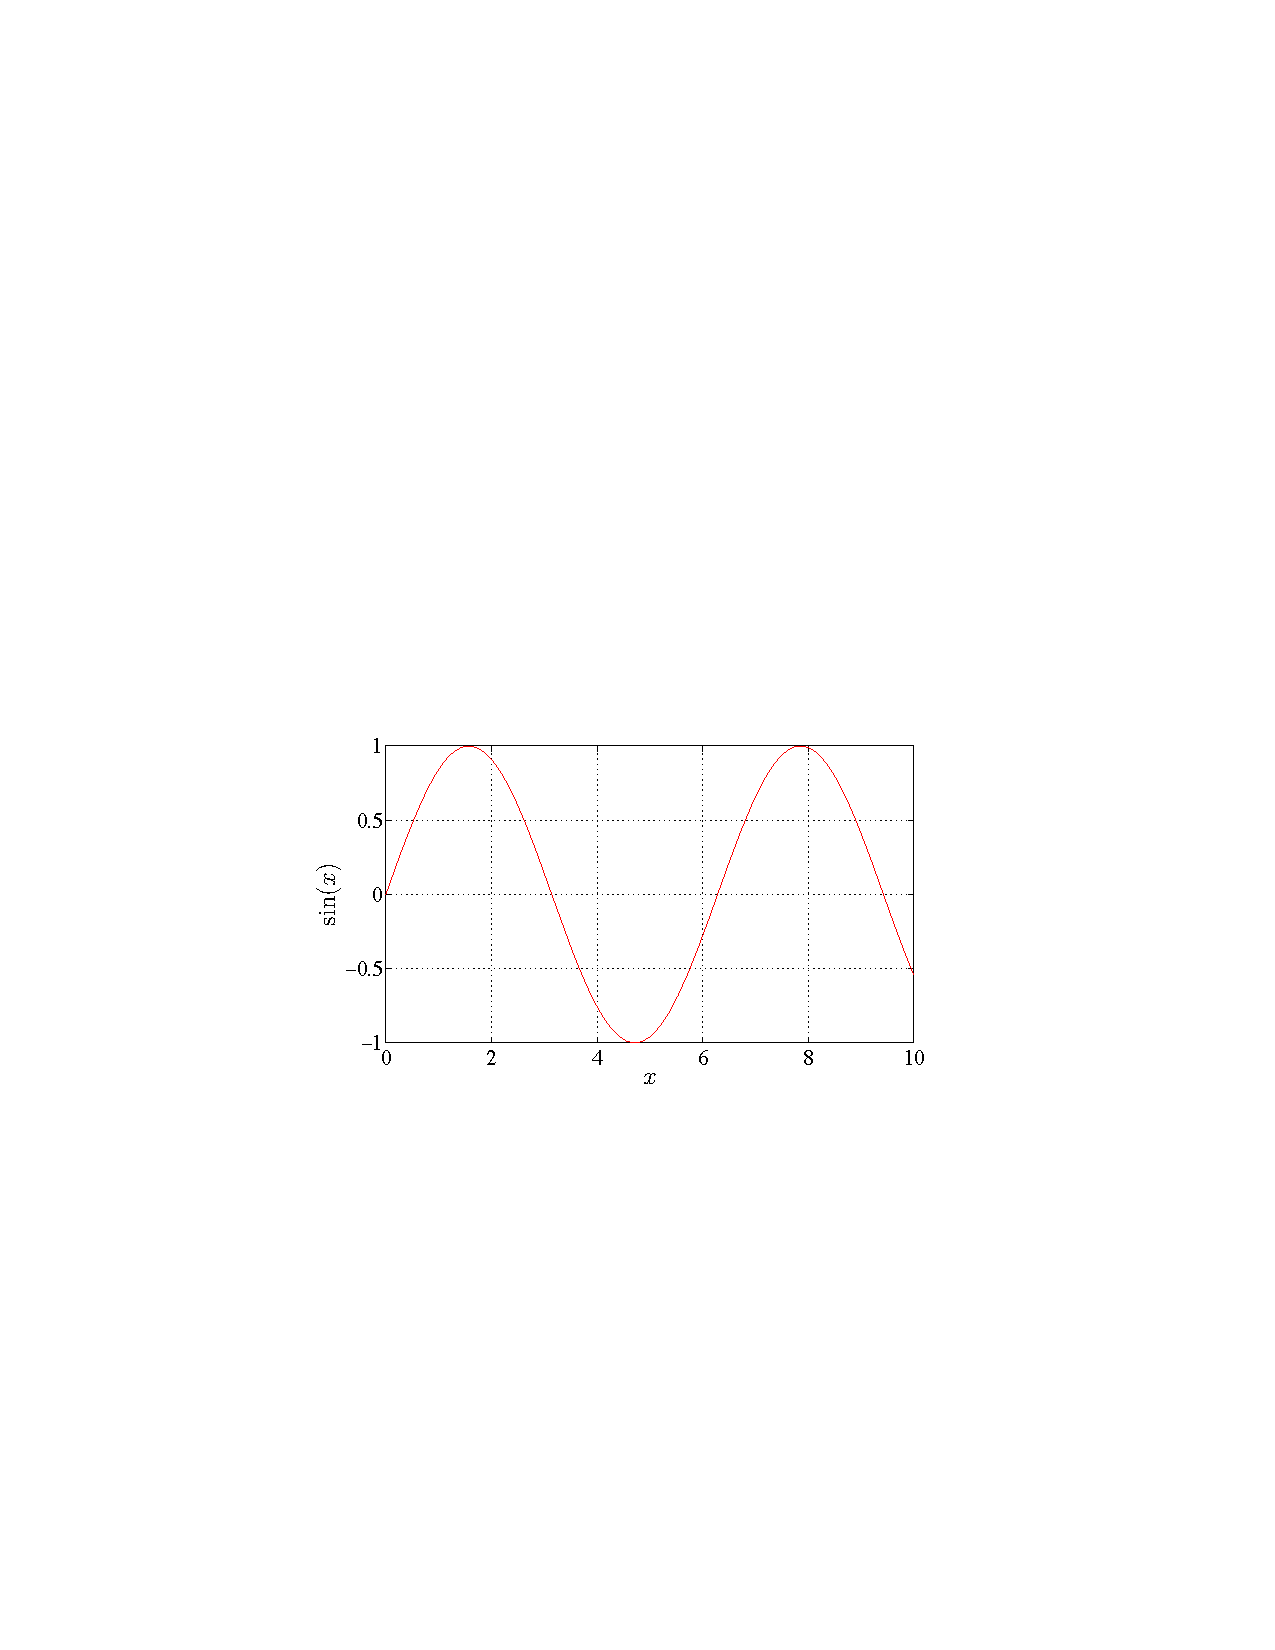
\includegraphics[width=\columnwidth]{fig1a}}
  \caption{Example of a figure with experimental results.}
  \label{fig:results}
\end{figure}

\section{Equations}
\label{sec:equations}

Equations should be placed on separate lines and consecutively
numbered with equation numbers in parentheses flush with the 
right margin, as illustrated in (\ref{eqn:wave_equation}) 
that gives the homogeneous acoustic wave equation in
Cartesian coordinates \cite{eWilliams1999},
\begin{equation}
  \label{eqn:wave_equation}
    \Delta^2p(x,y,z,t)-
    \displaystyle\frac{1}{c^2}\frac{\partial^2p(x,y,z,t)}{\partial t^2}=0,
\end{equation}
where $p(x,y,z,t)$ is an infinitesimal variation of acoustic 
pressure from its equilibrium value at position $(x,y,z)$ and 
time $t$, and where $c$ denotes the speed of sound.

Symbols in your equation should be defined before the equation 
appears or immediately following.  Use (1), not Eq. (1) or 
equation (1), except at the beginning of a sentence:  
``Equation (1) is ...''



\section{FOOTNOTES}
\label{sec:foot}

Use footnotes sparingly and place them at 
the bottom of the column on the page on which they are 
referenced. Use Times 9-point type, single-spaced. To 
help your readers, avoid using footnotes altogether and
include necessary peripheral observations in the text 
(within parentheses, if you prefer, as in this sentence).


\section{REFERENCES}
\label{sec:ref}

List and number all bibliographical references at the end 
of the paper. The references should be numbered in order 
of appearance in the document. When referring to them in 
the text, type the corresponding reference number in 
square brackets as shown at the end of this sentence 
\cite{cJones2003}, \cite{aSmith2000}. For \LaTeX\ users, 
the use of the Bib\TeX\ style file IEEEtran.bst is 
recommended, which is included in the \LaTeX\ paper 
kit available from the workshop website \cite{aaspweb}.

\section{ACKNOWLEDGMENT}
\label{sec:ack}

The preferred spelling of the word acknowledgment in 
America is without an ``e'' after the ``g.'' Try to avoid 
the stilted expression, ``One of us (R. B. G.) thanks ...''
Instead, try ``R.B.G.\ thanks ...''  Put sponsor 
acknowledgments in the unnumbered footnote on the first page.

% -------------------------------------------------------------------------
% Either list references using the bibliography style file IEEEtran.bst
\bibliographystyle{IEEEtran}
\bibliography{refsaasp}
%
% or list them by yourself
% \begin{thebibliography}{9}
% 
% \bibitem{aaspweb}
%   \url{http://www.elec.qmul.ac.uk/digitalmusic/sceneseventschallenge/}.
%
% \bibitem{IEEEPDFSpec}
%   {PDF} specification for {IEEE} {X}plore$^{\textregistered}$,
%   \url{http://www.ieee.org/portal/cms_docs/pubs/confstandards/pdfs/IEEE-PDF-SpecV401.pdf}.
%
% \bibitem{PDFOpenSourceTools}
%   Creating high resolution {PDF} files for book production with 
%   open source tools, 
%   \url{http://www.grassbook.org/neteler/highres_pdf.html}.
%
% \bibitem{eWilliams1999}
% E. Williams, \emph{Fourier Acoustics: Sound Radiation and Nearfield Acoustic
%   Holography}. London, UK: Academic Press, 1999.
% 
% \bibitem{ieeecopyright}
%   \url{http://www.ieee.org/web/publications/rights/copyrightmain.html}.
%
% \bibitem{cJones2003}
% C. Jones, A. Smith, and E. Roberts, ``A sample paper in conference
%   proceedings,'' in \emph{Proc. IEEE ICASSP}, vol. II, 2003, pp. 803--806.
% 
% \bibitem{aSmith2000}
% A. Smith, C. Jones, and E. Roberts, ``A sample paper in journals,'' 
%   \emph{IEEE Trans. Signal Process.}, vol. 62, pp. 291--294, Jan. 2000.
% 
% \end{thebibliography}


\end{sloppy}
\end{document}
